\section{Algorithmus}

	Da wir aus einer Matrix von Werten eine andere, gleich grosse  Matrix mit weiteren Werten berechnen, m�ssen wir zuerst diese Matrix in einen Vektor zerlegen.
	
	\begin{equation}
		\dunderline{A}\cdot \dunderline{X} \ne \dunderline{V} \qquad\Rightarrow\qquad \dunderline{A}\cdot \underline{x} = \underline{v}
		\label{eq:gleichung}
	\end{equation}
	
	Dabei haben wir bei beiden Matrizen die Spalten untereinander gereiht und so je einen Vektor mit der L�nge $n^2$ erhalten. Mathematisch macht das keinen Unterschied, solange wir am Schluss den L�sungsvektor wieder auf die selbe Art und Weise zu einer Matrix zusammenf�gen. Wir haben nun ein ganz normales lineares Gleichungssystem.
	
\[
	A=\left(
	\begin{array}{ccccc|ccccc|c|ccccc}
	    -4&     1&     0&\cdots&     0 &     1&     0&     0&\cdots&     0 &\cdots &      &      &      &      &      \\
	     1&    -4&     1&\cdots&     0 &     0&     1&     0&\cdots&     0 &\cdots &      &      &      &      &      \\
	     0&     1&    -4&\cdots&     0 &     0&     0&     1&\cdots&     0 &\cdots &      &      &     0&      &      \\
	\vdots&\vdots&\vdots&\ddots&\vdots &\vdots&\vdots&\vdots&\ddots&\vdots &       &      &      &      &      &      \\
	     0&     0&     0&\cdots&    -4 &     0&     0&     0&\dots &     1 &\cdots &      &      &      &      &      \\
	\hline
	     1&     0&     0&\cdots&     0 &    -4&     1&     0&\dots &     0 &\cdots &      &      &      &      &      \\
	     0&     1&     0&\cdots&     0 &     1&    -4&     1&\dots &     0 &\cdots &      &      &      &      &      \\
	     0&     0&     1&\cdots&     0 &     0&     1&    -4&\dots &     0 &\cdots &      &      &     0&      &      \\
	\vdots&\vdots&\vdots&\ddots&\vdots &\vdots&\vdots&\vdots&\ddots&\vdots &       &      &      &      &      &      \\
	     0&     0&     0&\cdots&     1 &     0&     0&     0&\cdots&    -4 &\cdots &      &      &      &      &      \\
	\hline
	\vdots&\vdots&\vdots&      &\vdots &\vdots&\vdots&\vdots&      &\vdots &\ddots &\vdots&\vdots&\vdots&      &\vdots\\
	\hline
	      &      &      &      &       &      &      &      &      &       &\cdots &    -4&     1&     0&\cdots&     0\\
	      &      &      &      &       &      &      &      &      &       &\cdots &     1&    -4&     1&\cdots&     0\\
	      &      &     0&      &       &      &      &     0&      &       &\cdots &     0&     1&    -4&\cdots&     0\\
	      &      &      &      &       &      &      &      &      &       &       &\vdots&\vdots&\vdots&\ddots&\vdots\\
	      &      &      &      &       &      &      &      &      &       &\cdots &     0&     0&     0&\cdots&    -4\\
	\end{array}
	\right) 
	\]
	
	Die Matrix $A$ enth�lt die Koeffizienten f�r die partielle Differentialgleichung 2. Ordnung, wie wir sie in der Vorlesung hergeleitet haben. Sie hat die Gr�sse $n^2 \times n^2$. Diese Matrix auf dem heap zu allozieren w�re f�r mittelgrosse Matrizen $V$ schon nicht mehr m�glich.
	
	
	
	Der ben�tigte Speicher f�r eine Matrix $V$ mit der Gr�sse $500 \times 500$ und float Werten (4 Byte) w�re
	
	\begin{equation}
		500^2 \times 500^2 \cdot 4\;\mathrm{Byte} = 232.8\;\mathrm{GByte}
	\end{equation}
	
	Mit $n = 1000$ sogar 3.64\;TByte, also definitiv zuviel. Um dieses Problem zu umgehen, errechnen wir die Koeffizienten f�r jeden Schritt einzeln, was mit kleinem Zeitaufwand m�glich ist da die Matrix $A$ d�nn besetzt ist.
	
	Da die diskrete partielle Ableitung jeweils nur die Elemente ober/unterhalb und links/recht des aktuellen Elementes in die Rechnung mit einbezieht, m�ssen mindestens $n$ Iterationen durchgef�hrt werden, damit sich das Potential �ber die ganze Ebene verteilt.
	
	\subsection{Parallelisierung}
		
		Um das Gleichungssystem (\ref{eq:gleichung}) zu l�sen, haben wir den Gauss-Seidel Algorithmus benutzt. Bei diesem Algorithmus ist, wie wir wissen, die aktuelle Zeile von der vorherigen abh�ngig. Bei der Parallelisierung wird das Gleichungssystem an verschiedenen Stellen zu l�sen begonnen. Das ist zwar nicht so effizient, wie ein "'normaler"' Gauss-Seidel, wird durch die Parallelisierung aber
		 schneller.
		
		Die Abweichung ist bei den ersten Schritten am gr�ssten, und wird bei jeder Iteration kleiner. Als wie die ersten Berechnungen durch gef�hrt hatten, fiel uns auf, dass die einzelnen Threads am Anfang gut als Linien von Spitzen sichtbar sind (\fref{fig:201_1}).
		
		\begin{figure}[h]
			\centering
			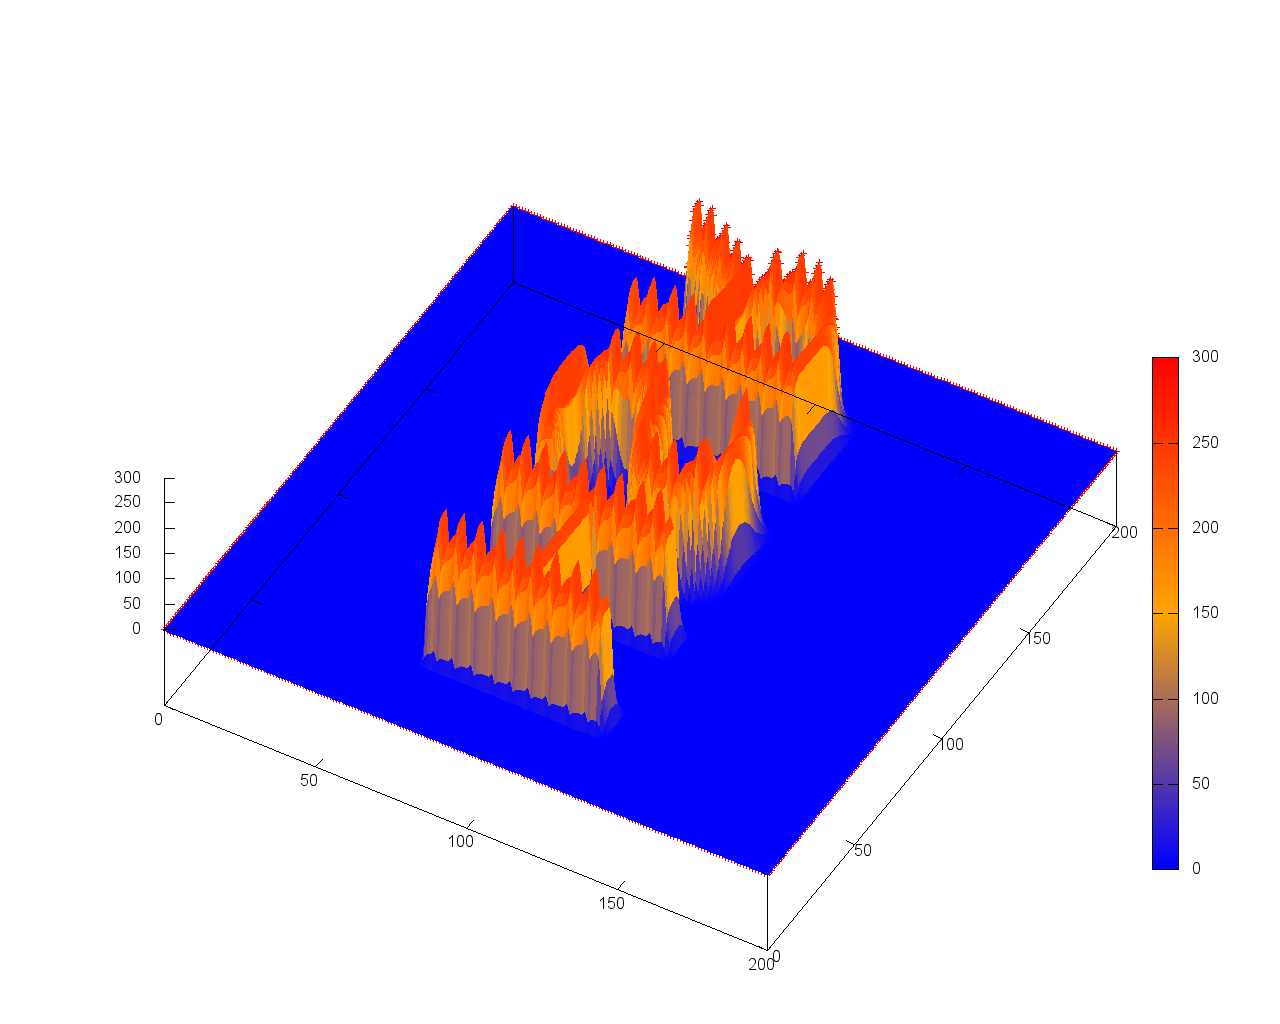
\includegraphics[width = 15cm]{./images/step001}
			\caption{Berechnung von einer $201 \times 201$ Fl�che mit 32 Threads nach dem ersten Iterationsschritt}
			\label{fig:201_1}
		\end{figure}
		
		
		Wir haben uns f�r OpenMP entschieden, da wir ein Grosses Problem haben, welches immer auf den selben Speicher zugreift. Wie schon beim Kugelsternhaufen erw�hnt, ist die Parallelisierung einfach zu realisieren:
		
\begin{code}
	int numthreads = 32;
	#pragma omp parallel for num_threads(numthreads)
		for (i = 0; i < dim; i++)
		{ ...
\end{code}

	\subsection{Probleme}
		
		Die Fl�che $f$ kann alle m�glichen Werte als Anfangsbedingung haben. Wir haben anfangs den  HSR-Schriftzug als FITS-File (Kapitel xxx) in eine Matrix 
% % % % % % % % % % TODO
		eingelesen. Der maximale Wert betrug anfangs nur 255,
		stieg nach einigen hundert Iterationen auf �ber 3000 an und die Funktion nahm die Form eines Haufen an. Wir hatten mit einem anderem Resultat gerechnet und �berpr�ften unseren Algorithmus. Wir konnten keinen Fehler entdecken und konnten die Werte mit MATLAB verifizieren. Die n�chste Frage war, ob der Gauss-Seidel konvergiert. Wir berechneten den Spektralradius der Matrix $A$ gem�ss Definition\;5.1 aus dem Skript HPC:
		
		\begin{eqnarray}
			A = M+N\\
			\varrho(M^{-1}N)<1
		\end{eqnarray}
		
		Da die Berechnung schnell sehr rechenaufwendig wird, man beachte, dass die Gr�sse der Matrix $A$ mit $n^4$ zunimmt, haben wir Matrizen mit kleinen $n$ berechnet. 	
		
		\begin{table}[h]
			\begin{tabular}{cc}
				n & Specktralradius $\varrho$\\\midrule
				5 & 0.7500\\
				10 & 0.92063\\
				15 & 0.96194\\
				20 & 0.97779\\
				25 & 0.98547\\
				40 & 0.99414
			\end{tabular}
			\centering
			\caption{Spaktralradien der Matrix $A$ f�r eine Matrix $f$ mit der Gr�sse $n\times n$}
		\end{table}

		Einerseits sind alle Werte kleiner Eins, was gut ist, andererseits sind die Werte sehr nahe bei Eins, was erkl�rt wieso unser Algorithmus so langsam konvergiert.

% % % % % % % % % % TODO Grosse Werte erkl�ren